% ===========================================================================
% Part XI - Non-Parametric Regression: GRNN (Experiment 19)
% ===========================================================================

\part{Non-Parametric Regression: Generalized Regression Neural Network}

% ---------------------------------------------------------------------------
\chapter{Experiment 19: Generalized Regression Neural Network (GRNN)}\label{exp:19}

\quickfacts
  {Dataset}{Real motorcycle impact data (\texttt{data/motorcycle.csv}, R \texttt{MASS::mcycle}); 133 observations, time vs head acceleration}
  {Key parameters}{GRNN from scratch (NumPy); smoothing spread $\sigma$ selected by 5-fold cross-validation over 0.02--1.0}
  {Headline result}{$\sigma$ = 0.08 (CV RMSE 25.00 g); held-out $R^2$ 0.7255, RMSE 22.78 g}

\section{Objective}
Implement GRNN-style kernel regression from scratch and study the effect of the smoothing
parameter $\sigma$ with cross-validation.

\section{Suggested Dataset}
Real motorcycle impact data (\texttt{data/motorcycle.csv}, R \texttt{MASS::mcycle}):
133 observations of time after impact (ms) versus head acceleration (g). Time is
standardized before computing kernel distances.

\section{Required Libraries}
numpy, pandas, matplotlib, scikit-learn (base classes, KFold, metrics).

\section{Brief Theory}
A GRNN has four layers: input, pattern, summation and output. With $N$ training points, each
pattern unit computes a Gaussian activation
\[
p_i(x) = \exp\!\left(-\frac{\lVert x - x_i \rVert^2}{2\sigma^2}\right),
\]
the summation layer accumulates $S(x) = \sum_i y_i\,p_i(x)$ and $D(x) = \sum_i p_i(x)$, and the
output layer returns the Nadaraya--Watson conditional mean
\[
\hat{y}(x) = \frac{S(x)}{D(x)}
           = \frac{\sum_i y_i \exp\!\left(-\lVert x-x_i\rVert^2 / 2\sigma^2\right)}
                  {\sum_i \exp\!\left(-\lVert x-x_i\rVert^2 / 2\sigma^2\right)} .
\]
Training is one-pass --- the model simply stores the data; prediction costs $O(N)$ per query.
The only hyperparameter is the smoothing spread $\sigma$: small values memorize noise (high
variance), large values over-smooth (high bias).

\section{Procedure}
\begin{enumerate}
  \item Load the motorcycle data and standardize the time feature.
  \item Implement the GRNN class (\texttt{fit} stores the data; \texttt{predict} computes the
        kernel weights).
  \item Visualize $\sigma = 0.05$, $0.25$ and $1.0$ (under- and over-smoothing).
  \item Select $\sigma$ by 5-fold cross-validation over $0.02 \ldots 1.0$.
  \item Refit on a 75\% split and evaluate the 25\% held-out set ($R^2$, RMSE).
\end{enumerate}

\section{Reference Implementation}
\begin{lstlisting}[style=mlcode,caption={GRNN prediction: pattern, summation and output layers}]
kernels = np.exp(-dist_sq / (2.0 * self.sigma ** 2))   # pattern layer
D = np.sum(kernels, axis=1)                            # denominator
S = np.dot(kernels, self.y_train_)                     # numerator
return S / np.where(D < 1e-12, 1e-12, D)               # output layer
\end{lstlisting}

\section{Evaluation / Expected Output}
\begin{table}[htbp]
  \centering
  \caption{GRNN on the real motorcycle impact data (133 observations).}
  \begin{tabular}{@{}lr@{}}
    \toprule
    \textbf{Item} & \textbf{Value} \\
    \midrule
    CV-selected $\sigma$ & 0.080 (CV RMSE 25.00 g) \\
    Train $R^2$ & 0.8073 \\
    Test $R^2$ & \best{0.7255} \\
    Test RMSE & 22.78 g (acceleration range $-134 \ldots +75$ g) \\
    \bottomrule
  \end{tabular}
\end{table}

\begin{figure}[htbp]
  \centering
  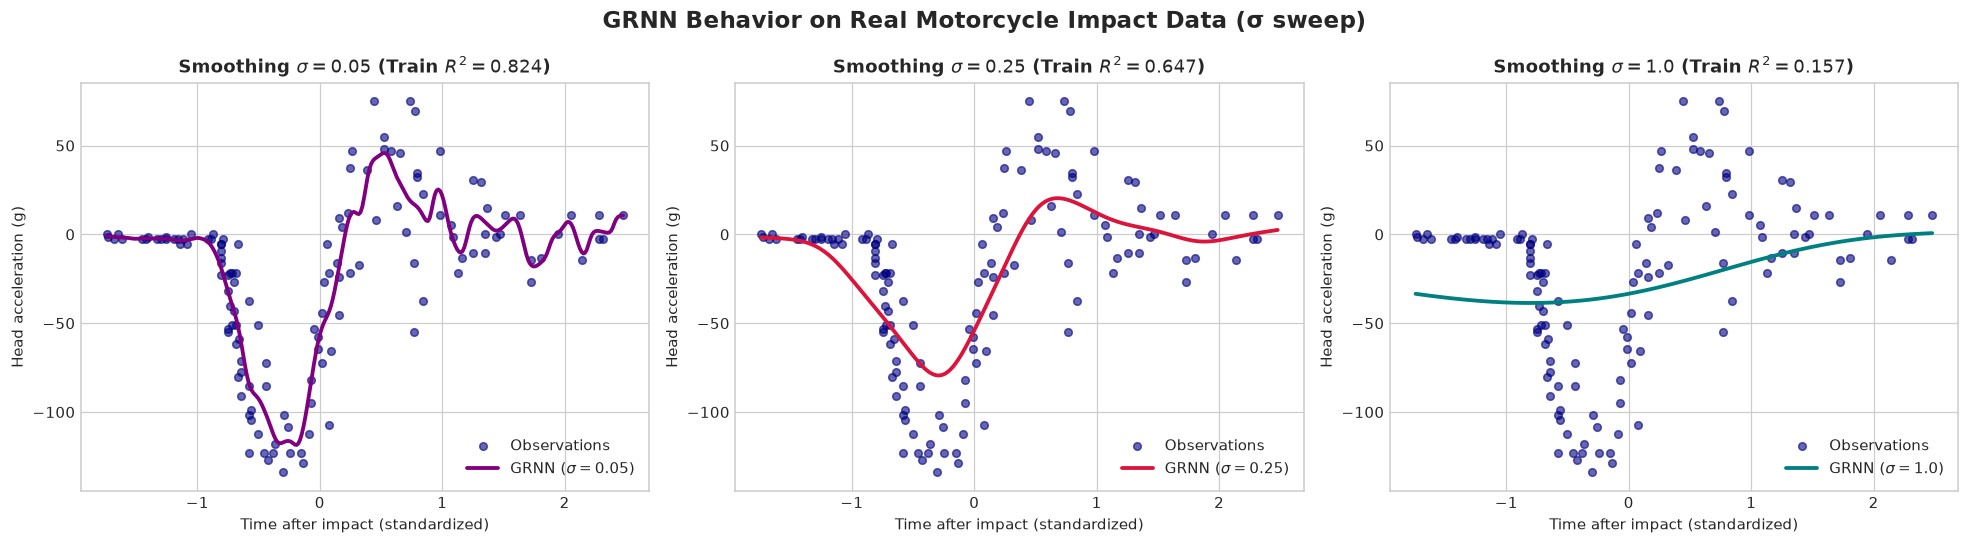
\includegraphics[width=0.98\textwidth]{figures/exp19_sigma_sweep.png}
  \caption{GRNN under different smoothing spreads on the motorcycle data: small $\sigma$
  follows noise, large $\sigma$ flattens the impact peak.}
  \label{fig:exp19-sigma}
\end{figure}

\begin{figure}[htbp]
  \centering
  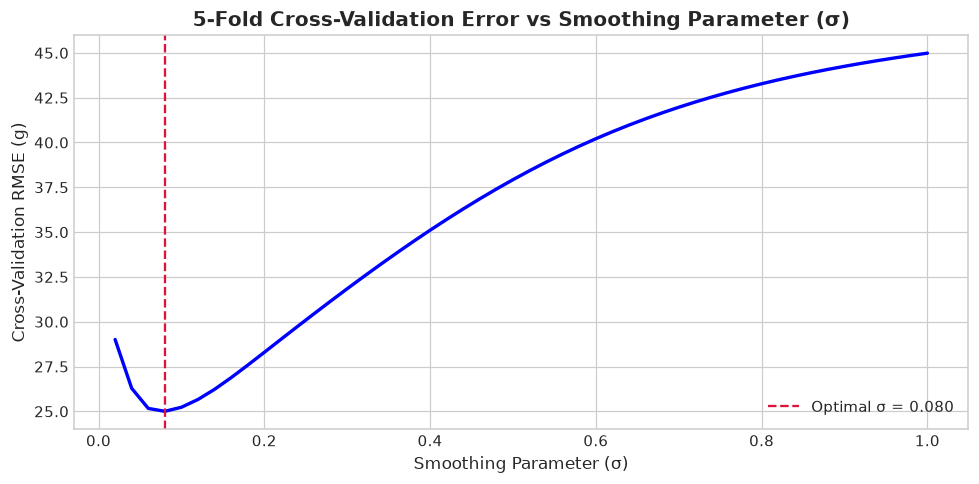
\includegraphics[width=0.72\textwidth]{figures/exp19_cv_curve.png}
  \caption{Five-fold cross-validation error versus $\sigma$; the clear minimum selects
  $\sigma = 0.08$.}
  \label{fig:exp19-cv}
\end{figure}

$\sigma = 0.05$ shows local wiggles (variance), while $\sigma = 0.25$--$1.0$ underfits the
sharp deceleration peak. On the smooth synthetic benchmark a GRNN reaches $R^2 \approx 0.95$;
on this real dataset the held-out $R^2$ is 0.73 because a single global $\sigma$ cannot be
simultaneously small at the impact discontinuity and large elsewhere. This is the classic
bias--variance limitation of global-bandwidth kernel regression; adaptive bandwidths or local
polynomial regression would improve it.

\section{Viva / Discussion Questions}
\begin{description}
  \item[Why is GRNN called non-parametric?] It does not learn a fixed set of parameters; the
  training data itself forms the model (memory-based kernel regression).
  \item[What does $\sigma$ control?] The smoothing bandwidth: small $\sigma$ fits noise (high
  variance), large $\sigma$ over-smooths (high bias).
  \item[How is GRNN related to kernel regression?] It is exactly the Nadaraya--Watson Gaussian
  kernel regression estimator of $\mathbb{E}[y \mid x]$, with one kernel per training
  observation.
  \item[Why is the test $R^2$ lower than on synthetic data?] The motorcycle data contains a
  near-discontinuity and an uneven measurement design, which a single global bandwidth cannot
  capture.
  \item[How would you improve the fit?] Use an adaptive or per-location bandwidth, local
  polynomial (LOESS) regression, or feature scaling plus anisotropic kernels.
\end{description}

\section{Complete Code Listing}
% ===========================================================================
% exp19_grnn.tex - complete code listings for Experiment 19
% Source: notebooks/11_generalized_regression_neural_network.ipynb (executed)
% ===========================================================================

\begin{codebox}[title={Core libraries}]
# ---- Core libraries ----
import numpy as np
import pandas as pd
import matplotlib.pyplot as plt
import seaborn as sns

from sklearn.base import BaseEstimator, RegressorMixin
from sklearn.model_selection import KFold, train_test_split
from sklearn.preprocessing import StandardScaler
from sklearn.metrics import r2_score, root_mean_squared_error

# Styling setup
plt.style.use('seaborn-v0_8-whitegrid' if 'seaborn-v0_8-whitegrid' in plt.style.available else 'default')
plt.rcParams['font.sans-serif'] = 'DejaVu Sans'
plt.rcParams['figure.figsize'] = (10, 6)
plt.rcParams['figure.dpi'] = 110
np.random.seed(42)
\end{codebox}

\begin{codebox}[title={GRNN class (from scratch)}]
class GRNN(BaseEstimator, RegressorMixin):
    """
    Generalized Regression Neural Network (Specht, 1991) - vectorized implementation.

    Prediction is the Nadaraya-Watson kernel regression estimate:
        y_hat(x) = sum_i y_i * exp(-||x - x_i||^2 / (2*sigma^2))
                 / sum_i     exp(-||x - x_i||^2 / (2*sigma^2))

    Training is one-pass: the model simply stores the training set (no gradient descent).
    The only hyperparameter is the smoothing spread sigma.
    """

    def __init__(self, sigma=1.0):
        self.sigma = sigma

    def fit(self, X, y):
        # "Training" = memorizing the data (pattern + summation layers)
        self.X_train_ = np.asarray(X, dtype=np.float64)
        self.y_train_ = np.asarray(y, dtype=np.float64).ravel()
        return self

    def predict(self, X):
        X_test = np.asarray(X, dtype=np.float64)

        # ---- Pattern layer: squared Euclidean distance between each test and train point ----
        # Uses the expansion ||a-b||^2 = ||a||^2 + ||b||^2 - 2 a.b for efficiency.
        dist_sq = np.sum(X_test**2, axis=1, keepdims=True) + \
                  np.sum(self.X_train_**2, axis=1, keepdims=True).T - \
                  2 * np.dot(X_test, self.X_train_.T)
        dist_sq = np.maximum(dist_sq, 0.0)  # guard against tiny negative values from rounding

        # ---- Pattern layer activation: Gaussian kernel of each training point ----
        kernels = np.exp(-dist_sq / (2.0 * (self.sigma ** 2)))

        # ---- Summation layer: D-sum (denominator) and S-sum (numerator) ----
        D = np.sum(kernels, axis=1)                 # unweighted sum of activations
        S = np.dot(kernels, self.y_train_)          # activation-weighted sum of targets

        # ---- Output layer: normalized weighted average (prevents 0/0 for isolated queries) ----
        D_safe = np.where(D < 1e-12, 1e-12, D)
        return S / D_safe


print("Custom vectorized GRNN class defined!")
\end{codebox}

\begin{codebox}[title={Load the real motorcycle impact data (MASS::mcycle)}]
# ---- Load the real motorcycle impact data (MASS::mcycle) ----
moto = pd.read_csv('../data/motorcycle.csv')
X = StandardScaler().fit_transform(moto['times'].values.reshape(-1, 1))  # time after impact (scaled)
y = moto['accel'].values                                                 # head acceleration (g)
print(f"Motorcycle data: {len(moto)} observations | time {moto.times.min()}-{moto.times.max()} ms | accel {moto.accel.min():.0f} to {moto.accel.max():.0f} g")

X_eval = np.linspace(X.min(), X.max(), 300).reshape(-1, 1)

# Under-smoothing, near-optimal, over-smoothing
sigmas = [0.05, 0.25, 1.0]
colors = ['purple', 'crimson', 'teal']

fig, axes = plt.subplots(1, 3, figsize=(18, 5))

for ax, sig, col in zip(axes, sigmas, colors):
    # Fit a fresh GRNN for each sigma (training is instant)
    grnn_demo = GRNN(sigma=sig).fit(X, y)
    y_pred_demo = grnn_demo.predict(X_eval)

    ax.scatter(X, y, color='navy', s=25, alpha=0.6, label='Observations')
    ax.plot(X_eval, y_pred_demo, color=col, lw=2.5, label=rf'GRNN ($\sigma={sig}$)')

    # Training R2 shows the bias-variance behavior for each sigma
    r2 = r2_score(y, grnn_demo.predict(X))
    ax.set_title(rf"Smoothing $\sigma = {sig}$ (Train $R^2 = {r2:.3f}$)", fontweight='bold')
    ax.set_xlabel("Time after impact (standardized)")
    ax.set_ylabel("Head acceleration (g)")
    ax.legend(loc='lower right')

plt.suptitle("GRNN Behavior on Real Motorcycle Impact Data (sigma sweep)", fontsize=15, fontweight='bold')
plt.tight_layout()
plt.show()
\end{codebox}

\begin{codebox}[title={5-fold CV grid search for the optimal smoothing sigma}]
# ---- 5-fold CV grid search for the optimal smoothing sigma ----
sigma_candidates = np.linspace(0.02, 1.0, 50)
cv_scores = []
kf = KFold(n_splits=5, shuffle=True, random_state=42)   # fixed folds for a fair comparison

for sig in sigma_candidates:
    fold_rmses = []
    for train_idx, val_idx in kf.split(X):
        # Split the data into this fold's train/validation parts
        X_tr, y_tr = X[train_idx], y[train_idx]
        X_va, y_va = X[val_idx], y[val_idx]

        # Fit GRNN on the training fold and score on the validation fold
        model = GRNN(sigma=sig).fit(X_tr, y_tr)
        preds = model.predict(X_va)
        fold_rmses.append(root_mean_squared_error(y_va, preds))

    cv_scores.append(np.mean(fold_rmses))   # average CV error for this sigma

best_idx = np.argmin(cv_scores)
best_sigma = sigma_candidates[best_idx]
print(f"Optimal Smoothing Parameter sigma: {best_sigma:.3f} (CV RMSE: {cv_scores[best_idx]:.4f} g)")

# ---- Plot the CV error curve and mark the optimum ----
plt.figure(figsize=(9, 4.5))
plt.plot(sigma_candidates, cv_scores, 'b-', lw=2.2)
plt.axvline(x=best_sigma, color='crimson', linestyle='--', label=f'Optimal sigma = {best_sigma:.3f}')
plt.title("5-Fold Cross-Validation Error vs Smoothing Parameter (sigma)", fontsize=13, fontweight='bold')
plt.xlabel("Smoothing Parameter (sigma)", fontsize=11)
plt.ylabel("Cross-Validation RMSE (g)", fontsize=11)
plt.legend()
plt.tight_layout()
plt.show()
\end{codebox}

\begin{codebox}[title={Final model: refit with the CV-selected sigma and evaluate on a held-out split}]
# ---- Final model: refit with the CV-selected sigma and evaluate on a held-out split ----
X_tr, X_te, y_tr, y_te = train_test_split(X, y, test_size=0.25, random_state=42)
final_model = GRNN(sigma=best_sigma).fit(X_tr, y_tr)
y_hat = final_model.predict(X_te)

print(f"Final GRNN with CV-selected sigma = {best_sigma:.3f}")
print(f" - Train R2:  {r2_score(y_tr, final_model.predict(X_tr)):.4f}")
print(f" - Test R2:   {r2_score(y_te, y_hat):.4f}")
print(f" - Test RMSE: {root_mean_squared_error(y_te, y_hat):.4f} g")
\end{codebox}

